\subsection{Frequency series fitting using mathematical optimization}
In this section, we will be discussing how to model frequency series using optimization methods.
In particular, we will discuss the fitting of noise spectum measurments in Sec.~\ref{sec:noise_modeling_baseline}, as a follow up of Sec.~\ref{sec:sensor_noise_measurement}.
And, the fitting of transfer function measurements is discussed in Sec.~\ref{sec:transfer_function_modeling}.
Some general tips on fitting frequency series using optimization is given in Sec.~\ref{sec:optimization_tips}.
In Sec.~\ref{sec:curve_fitting_examples}, we will exemplify the methods discussed.
We will be using mathematical optimization notations as given in appendix \ref{appendix:optimization}.
A good \verb|SciPy| reference on mathematical optimization can be found in \cite{scipy_mathematical_optimization}.
In this section, we will refer the word ``optimization'' to ``mathematical optimization'', which is to minimize an objective function/cost function.
\subsubsection{Noise spectrum modeling \label{sec:noise_modeling_baseline}}
In this section, we will discuss how to obtain a noise model from some sensor readout.
This can be useful if we need to have a analytic model or if we want to estimate the sensor noise from a signal sensor, whose readout is not purely noise-dominated.

If conditions in the Sec.~\ref{sec:displacement_sensors_baseline} and Sec.~\ref{sec:inertial_sensors_baseline}, such as fixing the suspensions or measuring the readout before installation, are not available, we cannot use the aforementioned noise measurement methods.
But, we can still estimate the sensor noise via a curve fitting procedure, if we have a noise model and if the signal sensor readout is not dominated at all frequencies, i.e. signal only dominates spectral partially.
An example of this situation would be a sensor that measures a damped sinusoidal, i.e.
\begin{equation}
	y(t) = x(t) + n(t) = C\Re{\left(e^{\sigma+i\omega_n t}\right)} + n(t)\,,
	\label{eqn:sensor_readout_damp_sinusoidal}
\end{equation}
where $x(t) = C\Re{\left(e^{\sigma+i\omega_n t}\right)}$ is the signal, $C$ is a real number, $\sigma$ is a negative real number, $\omega_n$ is the oscillation frequency, and $n(t)$ is the sensor noise.
In this case, the frequency spectrum of signal $x(t)$ is localized around $f=2\pi\omega_n$, while the frequency content of the sensor noise $n(t)$ spreads all frequencies, which is very typical for motion sensors in a suspension.

Say, we have measurements
\begin{equation}
	\hat{Y}(f) = \left[\hat{X}(f)^2 + \hat{N}(f)^2\right]^{\frac{1}{2}}\,,
	\label{eqn:sensor_measurement}
\end{equation}
where $\hat{Y}(f)$ is the ASD of the sensor readout $y(t)$, $\hat{X}(f)$ is the ASD of some signal $x(t)$, and $\hat{N}(f)$ is the ASD of the sensor noise $n(t)$ that we want to measure/model.
If we have a noise amplitude spectral model $\hat{N}_\mathrm{model}(f;\theta_{\hat{N}_\mathrm{model}})$, where $\theta_{\hat{N}_\mathrm{model}}$ is a list of parameters that defines the noise $\hat{N}_\mathrm{model}$, then we can do a curve fit to obtain the noise model.
A example choice of the noise model would be a quadrature sum
\begin{equation}
	\hat{N}_\mathrm{model}(f;\theta_{\hat{N}_\mathrm{model}})=\left[\left(\frac{N_a}{f^a}\right)^2 + \left(\frac{N_b}{f^b}\right)^2\right]^{\frac{1}{2}}\,,
	\label{eqn:noise_model}
\end{equation}
where $\theta_{\hat{N}_\mathrm{model}}=\{N_a,N_b,a,b\}$ are the model parameters.

The fit can be as simple as a least squares fit, i.e. by minimizing the sum of error squares cost function
\begin{equation}
	J_\mathrm{lsq}\mleft(\theta;A(m), B(m,\theta)\mright) = \sum_m^M\left[A(m)-B(m,\theta)\right]^2 w(m)^2\,,
	\label{eqn:least_squares_cost_function}
\end{equation}
where $\theta$ is some model parameters of an arbitrary analytical function $B(m,\theta)$, $A(m)$ is the measurement data, $m$ is a common parametrization of the series $A$ and $B$, and $w(m)$ is a user-designed weighting of each data point (weighting function).
Typical choices for $m$ could be time $t$, frequency $f$, or simply data index.
Minimization of Eqn.~\eqref{eqn:least_squares_cost_function} will give you the optimal parameters $\theta^*$ such that the best fit of data $A$ is the model $B(\theta^*)$.

We can use the least squares fit directly but this is not the best for fitting measurement data that is typically viewed in log or log-log plots, where the value of data points varies drastically in orders of magnitude.
Instead, we use $J_\mathrm{lsq}\mleft(\theta;\log{A(m)}, \log{B(m,\theta)}\mright)$.

As for the weighting function $w(f)$ (now as a function of frequency), an easy choice for our purpose would be
\begin{equation}
	w(f)=
	\begin{cases}
		0 &,\, f_\mathrm{lower}<f<f_\mathrm{upper} \\
		1 &,\, \textit{otherwise}
	\end{cases}
	\,,
	\label{eqn:weighting_function_frequency_bound}
\end{equation}
where $\left(f_\mathrm{lower},f_\mathrm{upper}\right)$ is a frequency bound that encloses frequency regions that has high SNR, indicated by the peak feature.
The choices of the design parameters $f_\mathrm{lower}$ and $f_\mathrm{upper}$ can't be easily told here as it requires users to look at the visualized data and make educated guesses.
Instead, we will demonstrate the choice of this bound in an example shown in Sec.~\ref{sec:curve_fitting_examples}.

To sum up, we have sensor data $\hat{Y}(f)$, which is an ASD (works for PSD as well.) as shown in Eqn.~\eqref{eqn:sensor_measurement}, and we would like to model the sensor noise $\hat{N}(f)$ with a model $\hat{N}(f;\theta_{\hat{N}_\mathrm{model}})$, where $\theta_{\hat{N}_\mathrm{model}}$ is a list of parameters of the sensor noise model.
We do so by minimizing the cost function
\begin{equation}
	\boxed{
		J_\mathrm{noise}\mleft(\theta_{\hat{N}_\mathrm{model}}\mright)=\sum_m^M\left[\log\hat{Y}(f_m)-\log\hat{N}_\mathrm{model}(f_m, \theta_{\hat{N}_\mathrm{model}})\right]^2 w(f)^2
	}\,,
	\label{eqn:noise_cost_function}
\end{equation}
where the weighting function $w(f)$ is given in Eqn.~\eqref{eqn:weighting_function_frequency_bound} and $f_m$ are the frequencies where the measured PSD and the model are evaluated.
The reason for using the log error $\log\hat{Y}(f) - \log\hat{N}_\mathrm{model}(f;\theta_{\hat{N}_\mathrm{model}})$ instead of the typical error is given in Sec.~\ref{sec:optimization_tips}, and will be obvious in the example section \ref{sec:curve_fitting_examples}.
Minimization gives best-fit parameters
\begin{equation}
	\theta_{\hat{N}_\mathrm{model}}^*=\arg\min{\theta_{\hat{N}_\mathrm{model}}} \hat{J}_\mathrm{noise}\mleft(\theta_{\hat{N}_\mathrm{model}}\mright)\,,
\end{equation} such that the noise model $\hat{N}_\mathrm{model}\mleft(f;\theta_{\hat{N}_\mathrm{model}}^*\mright)$ becomes a best fit of the noise spectral density $\hat{N}(f)$.
The minimization can be done using methods that will be discussed in Sec.~\ref{sec:optimization_tips}.
\subsubsection{Transfer function modeling \label{sec:transfer_function_modeling}}

\subsubsection{Some tips on using optimization \label{sec:optimization_tips}}
Minimization with measurement data can be done iteratively using optimization algorithms like gradient descent \cite{enwiki:1019572955} (local minimization) or stimulated annealing \cite{enwiki:1017509035} (global minimization).
We will not dive into the topic of mathematical optimization since it's a topic on it's own and is out of the scope of this document.
Instead, we will simply be using packages that are readily available.
A very useful Python submodule is \verb|scipy.optimize| \cite{scipy_optimize}.
It provides functions for both local minimization (\verb|scipy.optimize.minimize()|) and global minimization.
It comes with many popular algorithms such as the Nelder-Mead algorithm (\verb|scipy.optimize.minimize(..., method="Nelder-Mead")|) \cite{wiki:nelder_mead}, which is known to be good for optimization with noisy experiment data, or differential evolution \linebreak(\verb|scipy.optimize.differential_evolution()|) \cite{wiki:differential_evolution}.
The choice of algorithm is very subtle as different algorithms practically perform equally well for our purpose.
If you really need to know which one to use, try consulting \cite{scipy_mathematical_optimization}.
However, we do distinguish the choice between a local minimization algorithm and a global one.
The former can only be used when with guessed initial parameters, while the latter one can only be used when the boundaries of the parameters is known.
Typically, we\footnote{I mean I (Terrence)} prefer global optimization approaches because typically we don't know the parameters.
While the optimization result can depend on the initial guesses, having a poor guess would yield suboptimal results.

An important note on numerical optimization is parameter scaling \cite{wiki:preconditioner}.
We won't go into details.
The idea is to scale the parameters in such that they are all in the same scale, hence the cost function is equally sensitive to all parameters.
For some parameters $\theta=\{\theta_1,\theta_2\}$ that has a large dynamic range, it might be helpful if we optimize $\tilde{\theta}=\{\log\theta_1, \log\theta_2\}$ instead.
An example where this kind of rescaling is necessary is transfer function fitting with polynomial models, which have coefficients the vary in orders of magnitude.
Another example would be $N_a$ and $N_b$ from Eqn.~\eqref{eqn:noise_model}, which are noise levels that can also vary drastically.

Another useful pre-processing procedure would be to resample the data using an log-spaced frequency axis, instead of using the linearly spaced one as obtained during Fourier transform.
With linear-space frequency points, the majority of the data clusters at higher frequencies as viewed from a log-frequency axis, which create bias towards high frequency data.
As a result, the best-fit model might fit measurement data at higher frequencies better than that at lower frequencies.
A simple resample of the data will redistribute the data uniformly across the log-frequency axis.

\subsubsection{Examples \label{sec:curve_fitting_examples}}
\paragraph{Noise spectrum modeling}
Here, we will demonstrate how to use optimization to minimize cost functions \eqref{eqn:least_squares_cost_function} and \eqref{eqn:noise_cost_function} to model a sensor noise ASD $\hat{N}(f)$.
The notebook is available \href{https://kontrol.readthedocs.io/en/latest/tutorials/noise_spectrum_modeling_with_optimization.html}{here}.
We will assume a sensor readout $y(t)$ that follows Eqn.~\eqref{eqn:sensor_readout_damp_sinusoidal}, with a noise $n(t)$ that follows Eqn.~\eqref{eqn:noise_model}.
We will add measurement noise uniformly drawn from $[-3, 3]\,\mathrm{dB}$ to the sensor readout $y(t)$.

Fig.~\ref{fig:tutorialsnoisespectrummodelingwithoptimization10} shows the time series of the signal $x(t)$ and the frequency series $\hat{Y}(f)$, $\hat{N}(f)$, $\hat{X}(f)$, and the weighting function $w(f)$.
Here, the signal is
\begin{equation}
	x(t) = A\Re{\left(e^{\sigma+i\omega_n t}\right)},
\end{equation}
and we set $A=1$, $\sigma=-0.001$, $\omega_n=2\pi$.
The noise spectral density is
\begin{equation}
	\hat{N}(f) = \left[\left(\frac{N_{3.5}}{f^{3.5}}\right)^2+\left(\frac{N_1}{f^1}\right)^2\right]^\frac{1}{2}\,,
\end{equation}
where $N_{3.5}=\left(5\times10^{-7}\right)^\frac{1}{2}$ and $N_1=\left(1\times10^{-7}\right)^\frac{1}{2}$.
This these frequency dependencies ($-3.5$ and $-1$) are chosen to mimic the behavior of the geophone noise.
This kind of sensor noise profiles has large amplitude variations at different frequencies so it can be used as a benchmark problem for noise modeling.
So, the ASD of the sensor readout, in $\mathrm{dB}$ is
\begin{equation}
	20\log\hat{Y}(f) = 20\log\left[\hat{X}(f)^2 + \hat{N}(f)^2\right]^\frac{1}{2} + U(-3, 3)\,,
\end{equation}
where $U(a,b)$ is a random series drawn from a uniform distribution between $a$ and $b$.

In reality, the only information we have is the sensor readout $\hat{Y}(f)$, as given by the green curve shown in Fig.~\ref{fig:tutorialsnoisespectrummodelingwithoptimization10}.
From the plot, we see a peek feature around $0.7 ~ 2\,\mathrm{Hz}$, which indicates the presence of the signal $x(t)$.
This is something that we do not wish to model.
Hence, we set the weighting function
\begin{equation}
	w(f)=
	\begin{cases}
		0 & ,\,0.7<f<2\,\mathrm{Hz}\\
		1 & , otherwise.
	\end{cases}
	\,,
\end{equation}
so it filters out the part of the readout that we don't wish to model.
\begin{figure}[!h]
	\centering
	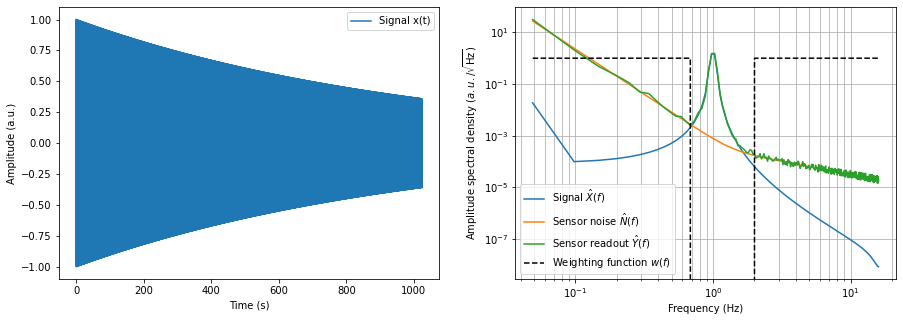
\includegraphics[width=1\linewidth]{figures/tutorials_noise_spectrum_modeling_with_optimization_1_0}
	\caption{(Left) Time series of the signal $x(t)$. (Right) Amplitude spectral densities of the readout $\hat{Y}(f)$, sensor noise $\hat{N}(f)$, signal $\hat{X}(f)$, and the designed weighting function $w(f)$.}
	\label{fig:tutorialsnoisespectrummodelingwithoptimization10}
\end{figure}

As for the model, we model ~\eqref{eqn:noise_model}.
We fit the measurement with 4 different configurations.
For the first two, we use least squares fit, which uses Eqn.~\eqref{eqn:least_squares_cost_function}, with model parameters $\theta_{\hat{N}_\mathrm{model}}=\{N_a, N_b, a, b\}$, and ``log parameters'' $\tilde{\theta}_{\hat{N}_\mathrm{model}}=\{\log N_a, \log N_b, a, b\}$, respectively.
For the other two, we use least squares fit with log error, which uses Eqn.~\eqref{eqn:noise_cost_function}, again with the two different sets of model parameters.
The motivation for using log parameters is discussed in Sec.~\ref{sec:optimization_tips}.


\begin{figure}[!h]
	\centering
	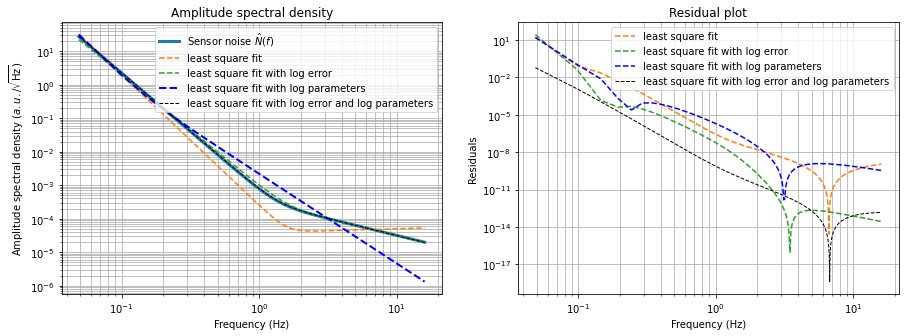
\includegraphics[width=1\linewidth]{figures/tutorials_noise_spectrum_modeling_with_optimization_8_0}
	\caption{(Left) Fitting results. (Right) Residuals, i.e. error squared.}
	\label{fig:tutorialsnoisespectrummodelingwithoptimization80}
\end{figure}

Fig.~\ref{fig:tutorialsnoisespectrummodelingwithoptimization80} shows the optimization results with the four configurations.
As can be seen on the left plot, least squares fit with log error yields noise models that fit the actual noise well across all frequencies.
But, the traditional least square fit fails at fitting the data at higher frequencies, where the amplitudes of the noise is orders of magnitude lower than that at lower frequencies.
Right plot in Fig.~\ref{fig:tutorialsnoisespectrummodelingwithoptimization80} shows the residuals, defined by the square error between the actual noise and the fit, of these four configuration.
As shown in the plot, modeling the noise with least square fit with log error and log parameters yields the best result in default settings.
This shows the importance in correct scaling of the model parameters.

For all these results, we used \verb|scipy.optimize.minimize()|, with default settings, to minimize the cost functions, and we start from an initial guess of $\{0, 0, 0, 0\}$ in all cases.
We emphasize that all these four configuration may perform equally well if we further tweak the optimization parameters in \verb|scipy.optimize.minimize()|, or using different optimization algorithms.
There are many optimization tweaks that can improve the fitting performance, but we won't discuss here.
The results shown in Fig.~\ref{fig:tutorialsnoisespectrummodelingwithoptimization80} only serves as a demonstration of how a careful design of the model and the cost functions can yield better results under the same settings.
